% \chapter{State of the art}
% \label{chap:state-of-the-art}
% \minitoc
\resetgraphicspath
\appendtographicspath{{./Introduction/figures}}
\appendtographicspath{{./Chapter 1/figures/} }
\appendtographicspath{{./Chapter 1/islands} }
\appendtographicspath{ {./Chapter 3/figures/erosion/}{./Chapter 3/figures/terrain_representations/}{./Chapter 3/results/}{./Chapter 3/otherPapersRepro/} {./Chapter 3/images/erosion-processes/}}

\chapter{Background}
\label{chap:background}
\minitoc

\section{Procedural terrain generation}
\label{sec:state-of-the-art_procedural-generation}

Procedural generation refers to algorithmically producing content rather than authoring it manually, leveraging rules, mathematical models, or data-driven methods. Its primary benefits include reducing storage needs (since content is generated on-the-fly), enabling rapid creation of large or varied content, and supporting both reproducibility and controlled variability. In terrain contexts, these advantages allow creation of vast landscapes or seascapes with relatively small parameter sets and facilitate interactive pipelines where artists or researchers can iterate quickly without storing every variant.

\AltTextImage{
    The conceptual roots of procedural techniques in graphics trace back to fractal geometry and noise functions. Mandelbrot's work on fractals demonstrated how complex, self-similar structures can arise from simple rules and randomness, influencing landscape modeling approaches that mimic natural roughness and multi-scale detail \cite{Mandelbrot1983}. Perlin's introduction of gradient noise provided a practical mechanism to generate coherent pseudo-random patterns for textures and terrain features \cite{Perlin1985}. These foundational ideas underpin many terrain algorithms, where noise at multiple scales produces hills, valleys, and finer details.
}{noises.pdf}{Example of procedural noises}{fig:intro-noises}

\AltTextImage{
    Procedural paradigms are often categorized as deterministic (repeatable given fixed inputs), stochastic (introducing randomness for variation), or hybrid (structure defined by deterministic rules, with randomness filling details). Rule-based systems, where content emerges via iterative application of predefined rules or grammars, also play a role, particularly in generating structured features (e.g., river networks, vegetation patterns). In terrain generation, deterministic components ensure global coherence (e.g., major landmass shapes), while stochastic elements add natural variability (e.g., subtle elevation perturbations). Later chapters leverage these paradigms: for instance, \cref{chap:coral-island}'s sketch-based island shape combined with noise and data-driven augmentation yields varied yet controlled outputs, and \cref{chap:semantic-representation}'s ecosystem simulation is governed by rule-based systems with stochastic sampling.
}{Snowflake5-Siertriangle11.jpg}{Fractal geometry: Sierpinsky Triangle in Koch Snowflack, from Larry Riddle}{fig:intro-fractal}

\AltTextImage{
    Recent advances incorporate machine learning to learn distributions of terrain patches or entire landscapes from data, enabling synthesis of realistic terrain patterns beyond hand-tuned noise parameters, using especially generative models like GANs or autoencoders. \cref{chap:coral-island} uses a conditional GAN to diversify coral island heightmaps. However, a detailed description of learning-based terrain methods appears in that chapter's State-of-the-Art.
}{Graph-coloring-Kim2020.png}{Rule-based graph coloring from \cite{Kim2020}}{fig:intro-rule-based-Kim2020}

In interactive and production pipelines, procedural systems must balance realism, speed, and user control. Fast evaluation (often parallelized and/or using GPU) supports real-time or near-interactive feedback for artist-driven editing. Parameter design and UI tools (e.g., sketching, semantic objects, masking) are critical to let users influence generation without overwhelming them. \cref{chap:semantic-representation}'s semantic \glosses{EnvObj} framework exemplifies user-centric design, enabling multi-scale editing and expert knowledge integration.

\AltTextImage{
    Procedural terrain generation also encompasses physical simulation techniques such as erosion and sediment transport models, that refine initial shapes to enhance plausibility. These simulations are typically more expensive but can run offline or via parallel algorithms. \cref{chap:erosion} presents a particle-based erosion method applicable across representations (height fields, voxels, etc.), reflecting this integration of procedural and physical approaches.
}{CFD-Sphynx.png}{Fluid simulation over the Great Sphynx}{fig:intro-cfd}






\section{Terrain representations}
Terrain refers to the physical features and configuration of a specific area of land. It includes the elevation, slope, and the overall topography, such as mountains, valleys, and plains. Terrain is often used to describe the surface characteristics of the land, focusing on the natural contours and the geographical aspects that define a region's physical form.

\AltTextImage{
    While the term "terrain" describes the physical characteristics of land, it does not include the natural elements that shape an area's identity. Elements like vegetation, water bodies, and climatic conditions, such as snow cover, are essential to how we perceive and understand a landscape. Therefore, when discussing procedural generation in virtual environments, "landscape generation" is a more fitting term, as it integrates these natural elements along with the topographical features.

    In addition to "terrain generation," other terms such as "landscape generation," "world generation," and "environment generation" can be used to describe the creation of virtual landscapes. These terms are interchangeable and can all refer to the process of generating physical terrain along with natural and artificial elements. However, by convention and for simplicity, the term "terrain generation" is most commonly used in the field. Despite its original focus on the physical features of the land, "terrain generation" has evolved to encompass a broader range of environmental elements, making it a convenient and widely accepted term for describing the comprehensive process of creating virtual environments.

}{Multi-representations-at-once-heightmap.png, Multi-representations-at-once.png}{An initial height map (top) can be converted in multiple terrain representations (bottom, from left to right): height field, layered model, density-voxel model (rendered with Marching Cubes), binary-voxel model}{fig:intro-multiple-representations}

    A terrain can be represented in various ways, each of them suited for a given application. In the different chapters of this thesis, we will move from one representation to another depending on the scope of the work, so we will only provide a short description of the representations used in this work. More details can be found in \cite{Galin2019}.

\subsection{Elevation models}

\begin{figure}[H]
    \centering
    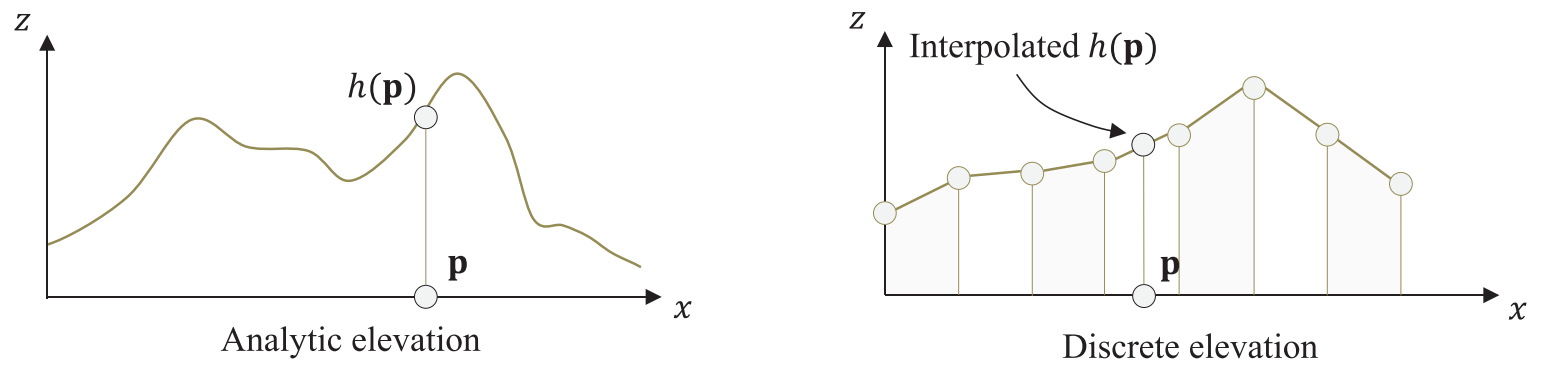
\includegraphics[width = 0.8 \linewidth]{elevation_representation.png}
    \caption{Elevation functions}
    \label{fig:erosion-elevation-representation}
\end{figure}

Elevation models are a fundamental approach in terrain representation, widely used in procedural generation due to their simplicity and efficiency. These models define the terrain as a function $h : \R^2 \to \R$, where each point in a 2D plane is mapped to an elevation value. This approach is particularly effective for representing terrains where the elevation is the only varying factor, such as hills, valleys, and plateaus, and it is best suited for terrains without complex 3D features like overhangs or caves. While we visualize elevation models in three dimensions, they are mathematically considered two-dimensional functions. In the domain of terrain generation, we will name them 2.5D models and are closely related to image processing.

Elevation models are widely used in industries where large-scale terrain representation is crucial. In video games, they provide the foundation for creating vast open-world environments. In geographic information systems (GIS) and remote sensing, height fields are used to represent real-world terrain data, offering a practical means of visualizing and analyzing geographical features. The ability to manipulate and control terrain features procedurally makes elevation models a common choice for applications that require efficient terrain generation and rendering.

They offer a powerful method for representing terrains in procedural generation, combining simplicity with flexibility. While they have limitations in representing complex 3D structures, their efficiency and compatibility with existing algorithms make them indispensable in a variety of applications.

\subsubsection{Implicit height fields}

\begin{wrapfigure}{L}{0.4\textwidth}
    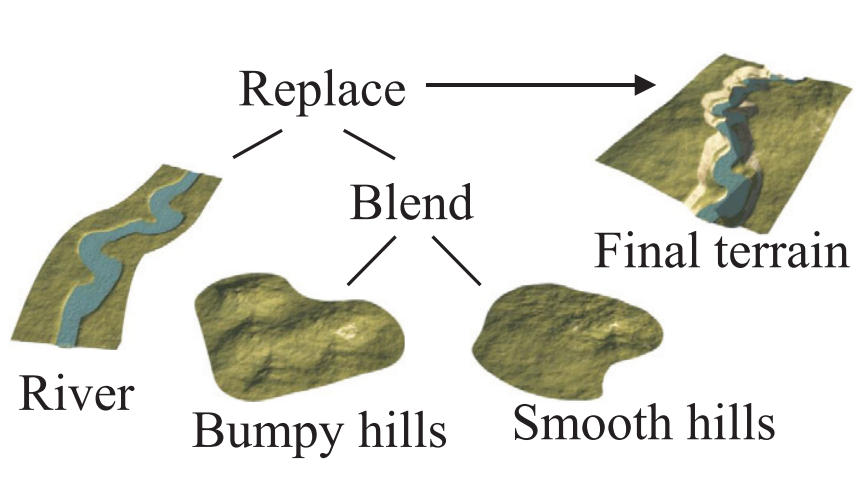
\includegraphics[width=\linewidth]{primitives_representation.png}
    \caption{Primitives composition}
    \label{fig:erosion-primitives-representation}
\end{wrapfigure}

Implicit height fields represent the terrain as a mathematical function that provides a height value at any given point in the domain. These functions can be procedural or closed-form expressions, allowing for compact storage and infinite precision in theory. The elevation function allows for easy manipulation of terrain features, making it ideal for generating terrains that require smooth, continuous surfaces. However, the primary disadvantage is the computational complexity involved in evaluating the function, especially for large or highly detailed terrains. The challenge lies in constructing functions that can realistically represent large-scale terrains with complex landforms.

This representation, inherently multi-scale from their mathematical nature, will be the main support for our \cref{chap:semantic-representation}'s environment generations.

\subsubsection{Discrete height fields}
Discrete height fields, or explicit height fields, are one of the most prevalent methods for terrain representation. These models consist of a 2D grid where each cell contains a height value, representing the elevation at that point. Height fields are particularly advantageous because they are simple to implement and are directly compatible with many rendering techniques and hardware, but also due to their closeness with image processing, a domain studied for many decades now. As the deep learning architectures used in \cref{chap:coral-island} are designed for image generation, the first contribution of this manuscript uses exclusively this representation.

The main advantage of height fields is their ability to handle large datasets efficiently, providing a balance between memory usage and detail. However, they are limited by their inability to represent terrains with overhangs or caves, as each point on the grid can only hold a single elevation value. Additionally, height fields often require interpolation methods, such as bi-linear or bi-cubic interpolation, to reconstruct a continuous surface from the discrete grid points. 

\subsection{Volumetric models}

\begin{figure}[H]
    \centering
    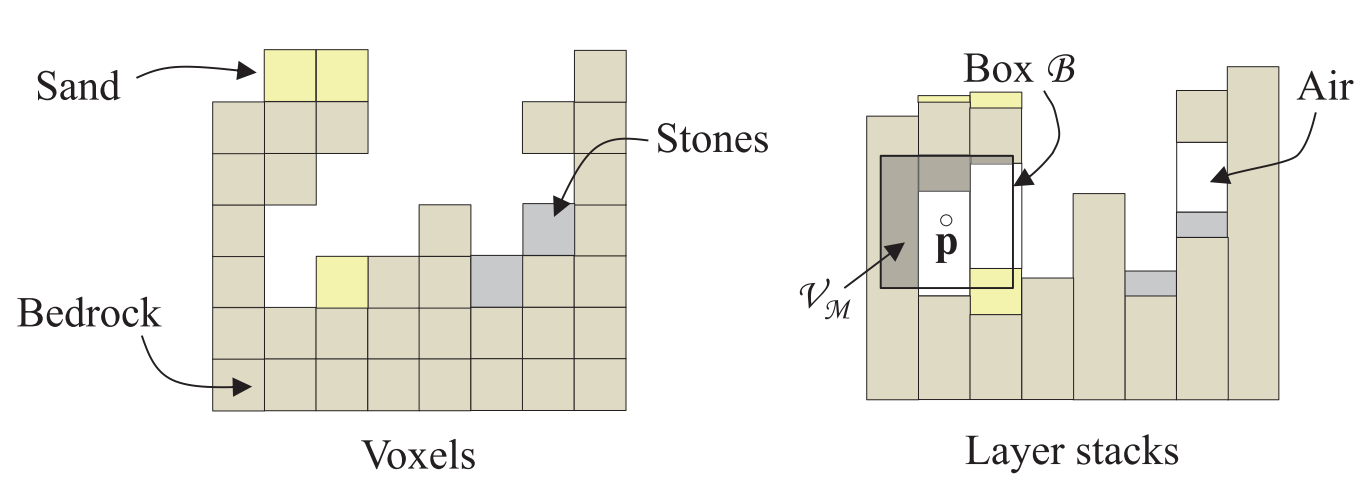
\includegraphics[width = 0.8 \linewidth]{volumetric_representation.png}
    \caption{Volumetric functions}
    \label{fig:erosion-volume-representation}
\end{figure}

Volumetric models represent a more complex approach to terrain modeling, allowing for the depiction of 3D features that go beyond the simple surface-based representation provided by elevation models. These models capture not only the surface of the terrain but also its internal structure, making them ideal for representing terrains with overhangs, caves, and other subsurface features. 

Volumetric models, including layered materials, voxel grids, and implicit models, are essential in applications where terrain complexity and detail are primordial. In geological simulations, these models allow for accurate representation of subsurface structures and processes. Voxel models are widely used in games that require dynamic terrain deformation, providing a rich interactive environment for players. Implicit models are favored in situations where smooth, continuous surfaces are needed, or require lightweight representation.

The erosion simulation presented in \cref{chap:erosion} evolves in the 3D space and will present applications for discrete and implicit volumetric representations.

\subsubsection{Implicit volumetric models}
\AltTextImageR{
    Implicit volumetric models describe the terrain's shape and features using an implicit function. The terrain is represented by a mathematical function $f: \R^3 \to \R$ that determines the terrain surface by evaluating to an isovalue, often zero. This function provides a continuous representation of the terrain, with points inside the terrain returning positive values and while points in the air evaluate to negative values. It allows for the seamless representation of complex terrain features, including caves, overhangs, and varying geological structures, which are impossible to represent with  elevation models.

    One of the key advantages of implicit models is their ability to produce smooth surfaces without the need for discrete polygonal meshes, which can result in realistic and natural-looking terrains. However, the computational complexity of evaluating the implicit function, especially for large terrains, can be a significant drawback. Additionally, converting an implicit surface into a mesh for rendering can be challenging and resource-intensive \cite{Araujo2015}.
}{Csg_tree.png}{Constructive Solid Geometry (CSG) uses boolean operators (union, intersection, difference) to construct 3D models. }{fig:intro-CSG}

\subsubsection{Layered models}
Layered models are a type of volumetric representation that encode different material layers within the terrain and are defined by a function $\mu : \R^3 \to \material$, where $\material$ denotes the material type at any given point in 3D space. This allows for a detailed representation of the terrain's internal composition, which can be crucial for applications requiring realistic geological simulations. Each layer is defined by its thickness or elevation, and multiple layers can be stacked to represent complex geological formations. These layers might include materials like bedrock, sand, soil, or water, each contributing to the overall structure of the terrain. Layered models are particularly useful in simulations that involve processes like erosion or sedimentation, where the interaction between different material layers affects the physical process.

\AltTextImage{
    The primary advantage of layered models is their ability to represent a stratified terrain with distinct material properties, which can be manipulated individually. This makes them well-suited for simulations that require detailed geological accuracy. However, they are more complex to implement than simple elevation models and require additional computational resources to manage the interactions between layers. 
}{Layer-representation.png}{Layer representation as described in \cite{Peytavie2009b}}{fig:intro-layers}



\subsubsection{Voxel grid models}
Voxel grids are a common method for representing 3D terrains in procedural generation, offering the ability to capture complex internal structures and features that are difficult or impossible to represent with surface-based models. In a voxel grid, the 3D space is divided into a regular grid of small, cube-shaped elements called voxels (volumetric pixels). Each voxel holds information about the material or properties of the terrain at that specific point in space. This approach allows for detailed modeling of features such as caves, tunnels, overhangs, and intricate underground networks. The regular grid structure allows for the use of image processing-oriented algorithms.

There are three primary types of voxel grids used in terrain representation: binary voxel grids, material voxel grids and density voxel grids. Each has distinct characteristics, advantages, and limitations, making them suitable for different applications. 

\subsubsubsection{Binary voxel grids}
Binary voxel grids are the simplest form of voxel representation. In these grids, defined $f: \R^3 \to \{0, 1\}$, each voxel is either "filled" or "empty," representing the presence or absence of material. This binary state is typically represented by a 1 (filled) or 0 (empty). Binary voxel grids are straightforward to implement and require much less memory compared to more complex voxel representations, making them ideal for applications where the primary concern is whether a space is occupied or not.

\AltTextImage{
    The simplicity of binary voxel grids is one of their main advantages. They are easy to understand and visualize, with each voxel requiring only a single bit of information to represent its state. Additionally, because only a binary state is stored, these grids can be memory-efficient when combined with compression techniques like Sparse Voxel Octrees (SVOs) \cite{Laine2010} or voxel Directed Acyclic Graphs (DAG) \cite{Villanueva2017,Careil2020}. The simplicity of the data structure also allows for quick processing, making binary voxel grids suitable for real-time applications where performance is required. However, the binary nature of these grids limits their ability to represent variations in material density or properties, or even smoothness, resulting in less detailed terrain models. This can lead to hard, blocky edges in the terrain, which may appear unnatural without additional smoothing or processing.
}{voxels-binary-density.png}{(Left) Binary voxel and (right) density voxel grids are encoded identically in a regular 3D lattice. The surface of binary voxel grid is most often presented as the faces of the filled cells in contact with empty cells, resulting in much more sharp edges compared to the isosurface of density voxels grids resulting from the Marching Cubes or Dual-Contouring algorithms. }{fig:intro-voxels-binary-density}


\AltTextImage{
    \subsubsubsection{Material voxel grids}
    Material voxel grids, defined as $\mu: \R^3 \to \material$, are commonly used in applications where simple occupancy information is sufficient. For example, voxel-based games like \citeProgram{Minecraft2011} utilize material grids to create terrains composed of solid blocks with clear boundaries. These grids are also employed in scientific simulations where the primary concern is the presence or absence of materials, rather than detailed material properties.
}{material-voxels-minecraft.png}{Each cell of the voxel grid is encoded with the identifier of a material. }{fig:intro-material-voxels-minecraft}

\subsubsubsection{Density voxel grids}
Finally, density voxel grids allow each voxel to store a range of values, representing varying degrees of material presence with $f: \R^3 \to \R$. Instead of a simple discrete state, a density voxel grid assigns a continuous value to each voxel, which can represent material density, opacity, or other properties. This added complexity enables density voxel grids to represent subtle variations in terrain, such as gradual changes in material density or smooth transitions between solid and empty spaces, allowing for more realistic and natural-looking terrain models.

% The use of density voxel grids results in soft transitions and smooth surfaces, reducing the blockiness typically associated with binary voxel grids. They are versatile and can represent not only solid terrain but also phenomena like fog, fluid densities, or temperature gradients. However, the increased detail and realism come at the cost of greater complexity. Density voxel grids require more memory and computational power, making them more challenging to implement and manage. The additional data and processing required can also lead to slower performance, particularly in real-time applications.

Density voxel grids are often used in high-fidelity simulations where detail and realism are essential. They are found in applications such as medical imaging, scientific visualizations, and advanced terrain modeling for films and visual effects. These grids are also employed in procedural terrain generation systems that require smooth and natural transitions between different terrain features, such as caves, cliffs, and eroded landscapes.




\section{Interactivity}
% \subsection{Realism-speed-control balance}
Procedural algorithms are designed to find a balance between three main objectives: controllability, realism, and computation speed.
In our work, we positioned our focus on the inclusion of the user in the generation process, resulting in a need to focus our attention on controllability for authoring without frustration, and computation speed in order to visualize results quickly, allowing to interatively interact with the system to obtain the best possible outputs. In this section we will briefly present the tools available for interacting with a procedural system.

Procedural terrain generation algorithms usually take parameters into account in order to generate something that fits the user's needs. The tools that let the user interact with the different parameters are essential to include efficiently the user in the process. 

The parameters that a user can play with can have many nature, and require a large varety of visual tools to interact with them. In the different nature of parameters, we can typically find: 
\begin{Itemize}
    \Item{Noise parameters:} Abstract values used in the equation ruling the noise functions. 
    \Item{Physical constants:} Constants that are used in physic simulations. They are often tweaked by the user to exagerate certain features, force some phenomena, etc... As they are constants, the parametrization of these values is often done inside the source code, as spinboxes, or inside a configuration file. 
    \Item{Densities and distributions:} Marking areas that are affected by a process, or where a seed can be used is useful to control a procedural algorithm. This is refered as "masking", but due to its binary nature, we can find sharp and unatural transitions from the use of binary masks. We often use weighted masks to provide more control about probabilities that a seed appear at one point. The control of the masks is usually done through grayscale images or by a "brush tool" that can modify the value directly on the surface of a 2D or 3D object. As virtual terrains are generally represented by a rectangular base, the use of brushes is a facade to the manipulation of a grayscale image.
    \Item{Structures placement:} Placing a specific terrain feature inside a terrain may be useful to finalize the generation of a landscape, or to add obstacles that will affect a physic simulation. This is usually implemented by clicking on the surface of the terrain, to provide the initial $xyz$ position, and then use translation and rotation tools to adjust the placement. If many elements are added, we usually use the previous strategy, involving masking, to add all the structures.
    \Item{Manual manipulation of the terrain:} In order to customize at a lower level the surface of the terrain, the user may be able to alter the surface of the terrain by using brushes. Clicking or dragging a brush on the surface usually result in the rise or lowering of the surface level around the brush. This process modifies the field representing the terrain. Procedural brushes can imply more complex behaviours, and may use the velocity of the brush stroke in its input.
\end{Itemize}

Each developer uses different strategies for each type of parameters as the needs or objectives of each application is different. Providing the user with too many parameters can be overwhelming, while too few can limit the output possibilities. In the meantime, providing unintuitive parameters like dimensionless values often result in trial and error strategy, requiering to run the generation algorithm many times before finding the appropriate values. This implies that the algorithms must be able to be executed fast. On an opposite side, removing some user controls to use hard-coded constants instead can greatly increase the speed. Finally, an algorithm that aims to be fast or let the user many parameters to control may reduce the realism of the output. Most algorithms try to strike a balance between realism, speed and control.

% User interaction affects how users balance realism, speed, and control over generated content.

Realism refers to the extent to which generated content accurately represents real-world characteristics, such as visual details, physical processes, and natural patterns. This is especially important in simulations, visualizations, and training environments where physical accuracy is critical. Techniques to enhance realism include physical simulations, which model processes like erosion and sediment transport, and the integration of expert knowledge from fields such as geology and ecology. However, achieving realism can be challenging due to the complexity of detailed simulations and the need for specialized expertise, which can demand substantial computational resources and inputs. Usually, a realistic algorithm tends to have low user control and speed.

On another hand, speed is about the efficiency of content generation within acceptable time constraints. While no official categorisation has been set, James Gain proposed to describe levels of speed based on response time:
\begin{Itemize}
    \Item{Real-time:} generation in less than 30 milliseconds, essential for interactive applications like VR environments. 
    \Item{Interactive:} generation in under 3 seconds, suitable for user-driven customization in games and simulations. 
    \Item{Near-interactive:} generation in less than 5 minutes, applicable for larger-scale simulations where some delay is acceptable. 
    \Item{Offline:} generation that takes longer, often used for precomputed content or offline rendering.
\end{Itemize}

The execution speed of a procedural algorithm is crucial as the user will fine-tune the parameters before being satisfied.
Optimizing speed involves using efficient algorithms and parallel processing. Almost all recent works achieve fast execution time thanks to high parallelisation on GPU. Other types of algorithm may rely on a refinement paradigm, generating a coarse result at first and then iteratively adding finer details, such that the global output shape is available long time before the real final result.

Control refers to how much users can influence or direct the procedural generation process to meet their specific needs or preferences. This includes parameters fine-tuning, allowing users to modify parameters like the noise functions parameters or the simulation parameters, and artistic control tools, made for artists and designers, to guide the generation process with the use of masks and brushes, allowing for combination and mixing of different algorithms.

Managing diverse and sometimes conflicting user expectations, such as balancing creative freedom with the demand for realistic outcomes, requires careful consideration. Additionally, it is essential to balance the complexity of procedural systems to ensure they remain user-friendly, avoiding overwhelming users or producing results that feel artificial or inconsistent.




\section{Underwater landscapes}
Underwater landscapes, or "seascapes", encompass the complex and dynamic terrains found beneath the ocean surface. Unlike landscapes above water level, we will call "aerial landscapes", these environments are shaped not only by geological forces but also by biological activity, hydrodynamic processes, and chemical interactions. Coral reef islands represent a particularly intricate subset of these environments, where the terrain is actively constructed and modified by living organisms, primarily reef-building corals. The spatial and structural complexity of such systems, which span multiple scales from individual coral polyps to entire reef platforms, poses unique challenges for their representation and simulation.

In the context of procedural terrain generation, the modeling of underwater landscapes demands fundamentally different assumptions and techniques from those used for land-based terrains. The submerged setting alters the influence of gravity, light, and fluid dynamics, while also introducing significant observational constraints. Furthermore, the scarcity of high-resolution and volumetric data capturesing the structural complexity and biological processes of coral reef systems poses a major challenge for data-driven or example-based modeling approaches. In this context, procedural generation offers an alternative by synthesizing underwater landscapes from first principles, guided by interdisciplinary understanding of geological, biological, and hydrodynamic processes. This section reviews the key environmental, observational, and modeling challenges associated with seascapes, with a focus on those that motivate and constrain procedural terrain generation for coral reef island systems.

\subsection{Physical environment differences}
The underwater environment differs fundamentally from terrestrial settings in the physical forces that shape landscape formation, the conditions for biological growth, and the constraints imposed on sensing and modeling. These differences directly impact the assumptions underlying terrain generation and limit the applicability of methods developed for aerial landscapes.

First, while gravity remains a dominant force in geomorphological evolution, provoking sediment transport and slope stability, buoyancy significantly alters the behavior of materials and organisms underwater. The net effect is a reduction in apparent weight and in gravity-driven surface processes, particularly at smaller scales, where water movement becomes a more dominant shaping force. Hydrodynamics plays a central role in shaping the morphology of coral reef systems by redistributing sediments, constraining reef growth zones, and sculpting reef edges and channels [Lowe, 2015].

Second, the optical properties of seawater introduce strict environmental constraints. Light attenuation limits the availability area for photosynthesis, which in turn defines vertical growth boundaries for reef-building corals [Huston, 1985]. It also constrains the applicability of remote sensing and optical measurement techniques, limiting their effectiveness to shallow, clear-water environments.

Third, underwater terrains are shaped not only by physical processes but also by active biological construction and destruction. Reef-building organisms contribute directly to topographic complexity through accretion, while bioeroder species like parrotfish, sponges, and urchins actively degrade and remodel the substrate [Perry, 2012]. % These biological processes introduce temporally variable and spatially heterogeneous modifications to the seascape that are difficult to capture with conventional terrain modeling frameworks.

Finally, these coupled physical-biological interactions result in terrain features that are not only highly complex, but also scale-dependent and dynamic. Overhangs, cavities, and porous structures restrict standard heightmap-based representations. Moreover, many features emerge from feedback loops between hydrodynamics, sedimentation, and biological growth, further complicating attempts to generalize aerial terrain modeling techniques to underwater environments. % For these reasons, the procedural generation of coral reef landscapes must be grounded in an understanding of the unique environmental dynamics that govern their formation.


\subsection{Observation and 3D data acquisition challenges}
Despite the growing interest in seafloor mapping, high-resolution, volumetric datasets of coral reef environments remain scarce. Most available data are limited to bathymetric or altimetric surface representations, typically acquired through sonar or satellite-derived methods, which offer only 2.5D elevation maps and lack information on vertical and sub-surface complexity. Features such as overhangs, internal cavities, and fine-scale biological structures are not captured, limiting the fidelity of directly observed data.

Furthermore, the availability of optical or active remote sensing techniques, such as underwater photogrammetry or bathymetric LIDAR, is restricted to shallow and optically clear waters, and risk-free zones for the diver or robot supporting the sensor. These methods are ineffective in turbid or deep environments, which characterize large portions of reef systems, particularly mesophotic and fore-reef zones. Consequently, consistent 3D coverage across depth gradients is virtually unattainable with current technology.

In situ surveys are often constrained by logistical, financial, and environmental factors. Diver-based surveys, while effective at fine scales, are labor-intensive, spatially limited, and can disturb local fauna, thereby introducing bias in biological assessments. Remotely operated vehicles (ROVs) offer greater depth access but require tethering and constant supervision. Autonomous underwater vehicles (AUVs), by contrast, have shown promise in collecting low-disturbance imagery and acoustic data in a more scalable manner \cite{Gonzalez-Rivero2016} [González-Rivero et al., 2020], and represent a potential pathway for systematic 3D surveying in the future.


\subsection{Environmental dynamics and interdisciplinary integration}
% Geological and sedimentary frameworks
Coral reef terrains develop in relation with underlying geological structures and sedimentary processes. Substrate stability and morphology are governed by sediment supply which controls the distribution of fine sediments in lagoons versus coarser rubble zones on reef fronts [Montaggioni, 2005]. Tectonic uplift or subsidence modulates relative sea level, determining exposure intervals that drive the formation of reef terraces and platform architecture \cite{Hopley2014} [Hopley, 1982]. Geomorphologic events, such as submarine landslides or turbidity currents on reef slopes, and wave-driven abrasion, further reshape bathymetry at meso- to macroscale.

% 4.3 Hydrodynamic controls and feedbacks
Hydrodynamic regimes highly influence sediment transport, mechanical stress, and ecological viability in reef environments. Persistent currents and wave action determine patterns of erosion and deposition on slopes and flats, shape reef crests, and drive overtopping and flushing in lagoonal areas [Lowe \& Falter, 2015]. Episodic storms or large swell events can produce rapid morphological change via scour, sediment redistribution, and coral breakage, punctuating longer-term growth trajectories. Crucially, the evolving reef morphology modifies local flow fields which in turn influence subsequent sediment dynamics and biological processes. %For procedural modeling, simplified representations of these feedback loops (for example, depth- and form-dependent growth constraints) are necessary to generate plausible reef shapes without resorting to full CFD coupling.

% Reef-building organisms actively generate topographic complexity through species-specific growth forms and rates, while other biota erode and remodel the substrate. Scleractinian corals display branching, massive, or encrusting morphologies, each with distinct accretion dynamics influenced by light availability, water clarity, and nutrient fluxes that establish vertical zonation [Huston, 1985; Anthony \& Fabricius, 2000]. Concurrently, bioeroders—such as parrotfish, boring sponges, and sea urchins—and mechanical disturbances from storms produce cavities, rubble, and heterogeneous surface textures [Perry et al., 2012]. Successional trajectories after disturbance further affect spatial patterns over years to decades, as pioneer species give way to longer-lived taxa, and physical structure influences recruitment. The emergent reef architecture, in turn, alters local hydrodynamics, attenuating flow or generating eddies, which feeds back into larval settlement and nutrient exchange [Falter et al., 2004]. These intertwined accretion-erosion dynamics complicate the assumption of static terrain templates and must inform any procedural synthesis.

% Biological construction and degradation
Parallely to erosion processes generated through geological, climatic and hydrological events, the organic nature of coral reef continuously remodel and regenerate the substrate. 
% 4.4 Chemical and physical environmental drivers
However, abiotic factors such as light attenuation, temperature regimes, and water chemistry constrain both biological growth and sedimentary behavior. Attenuation by turbidity and depth limits photosynthesis, setting depth boundaries for coral accretion [Kirk, 1994]. 
% Temperature and pH affect calcification rates and bleaching susceptibility, influencing long-term growth patterns and resilience under climate change. 
Nutrient concentrations from terrestrial runoff can shift community composition toward macroalgae or favor coral health, while turbidity governs sediment deposition on reef surfaces. % Procedural frameworks built from first principles must encode these environmental limits (e.g., depth-dependent growth probability, maximum accretion rates under given temperature regimes) even when direct observational data are unavailable.

% 4.5 Data heterogeneity, uncertainty, and integration
Integrating geological, ecological, hydrodynamic, and chemical knowledge effectively implies the reconciling diverse data types and spatiotemporal resolutions. Geological information often spans over millennial time scales and kilometer space scale, whereas ecological observations like colony growth rates are studied in years and counted in meters; hydrodynamic models and sensor time series each have their own spatiotemporal resolutions. % Data formats vary from bathymetric DEMs and point clouds to ecological transect datasets and model outputs, requiring consistent georeferencing (horizontal and vertical datums) and adherence to metadata standards. Many reef areas lack comprehensive surveys, so proxy parameters or analog-derived values (for accretion rates, sedimentation) must be adopted with explicit uncertainty bounds. Effective integration thus relies on interdisciplinary collaboration to translate domain knowledge into generative constraints and to select simplified parameterizations that remain computationally tractable. Explicit representation of uncertainty—via parameter ranges or scenario ensembles—helps ensure that procedural outputs acknowledge their assumptions.

% 4.6 Procedural relevance and synthesis
The complex, dynamic nature of reef environments motivates process-informed procedural generation rather than example-based interpolation. Algorithms should embody process-based constraints such as depth-dependent accretion limits, susceptibility to storm-induced degradation, and form-flow feedbacks while allowing staged synthesis to yield realistic structural patterns. Simplified feedback loops, such as adjusting local growth likelihood based on simulated flow attenuation, can capture essential interactions without full physical simulation. Given data scarcity, procedural outputs should support exploration across parameter spaces or alternative scenarios, making assumptions transparent. % Validation can rely on general empirical observations (e.g., known zonation profiles, typical reef cross sections) and expert judgment to assess plausibility in the absence of dense ground-truth data.



\subsection{Procedural modeling challenges}
\citep{ParisThesis} classified the different geological structures in four different spatial scales: the \textit{megascale} describes landforms spread on more than \si{100}{km} such as continents or mountain ranges, the \textit{macroscale} between \si{1}{km} and \si{100}{km} like islands, rivers or cave networks, the \textit{mesoscale} ranging from \si{10}{m} to \si{1}{km} contains most complex structures (arches, ravines, cliffs, ...) and finally the \textit{microscale} for features between \si{10}{cm} and \si{10}{m}, like sand ripples, ventifacts, rocks, etc. Generally, we consider as \textit{large-scale} features that can be seen from far away and \textit{small-scale} elements for which somebody has to be to close to to observe it.

% 5.1 Multi-scale structure and level-of-detail
Coral reef island landscapes exhibit structural complexity across scales ranging from millimeter- to kilometer-scale features, and procedural generation must accommodate seamless transitions among these scales. At the microscale, individual coral morphologies, crevice networks, and sediment textures determine fine habitat details, whereas at the mesoscale, colony aggregations, reef crests, and lagoon basins define intermediate morphology. Macroscale features include the overall platform shape, island emergence, and large geomorphic structures such as reef rims or terrace outlines. 


% A procedural framework must thus employ hierarchical or level-of-detail (LOD) strategies—such as multi-resolution meshes or adaptive tessellation—to allocate computational resources appropriately: generating high-fidelity detail only where needed (e.g., near observer or for ecological relevance) while relying on coarser representations elsewhere. Parameterization of procedural detail (e.g., fractal noise amplitudes, colony size distributions) should be informed by empirical statistics or domain knowledge to avoid unrealistic patterns when scaling between levels.

% % 5.2 Generating full 3D structures beyond surface terrain
% Unlike aerial heightmaps, reef environments contain overhangs, cavities, and porous frameworks created by biological accretion and bioerosion. Procedural methods must therefore synthesize plausible volumetric geometry rather than relying on 2.5D surfaces. This can be achieved through combinations of rule-based solid modeling (e.g., L-systems for branching coral forms; Prusinkiewicz \& Lindenmayer, 1990), constructive solid geometry (CSG) or volumetric grammars, and stochastic placement of voids to mimic bioerosion. For example, a procedural pipeline may first establish a coarse scaffold for reef framework (informed by depth-dependent envelope shapes) and then instantiate volumetric modules representing coral colonies or cavities according to ecological rules. Such methods must ensure topological consistency (avoiding non-manifold geometry) and maintain computational tractability, for instance by representing fine-scale porosity via procedural textures or voxel-based approximations in localized regions.

% % 5.3 Ecologically informed growth and degradation
% Process-informed generation relies on encoding ecological constraints and interactions. Coral growth algorithms may simulate accretion under depth- and light-dependent rules, with branching or massive morphologies chosen according to environmental parameters (e.g., light attenuation, nutrient flux). Agent-based or rule-based models can represent competition for space, where faster-growing but fragile forms may dominate in sheltered zones, whereas robust morphologies persist in high-energy areas (Anthony \& Fabricius, 2000). Simulated bioerosion events—modeled as probabilistic removal of material in regions exposed to bioeroder activity or storm damage—introduce heterogeneity and temporal variability. Although full temporal simulation may be computationally expensive, staged synthesis (e.g., iterative growth phases punctuated by disturbance routines) can yield realistic geometry. Embedding simplified feedback—such as reducing local growth probability in regions where procedural “flow attenuation” indicates low circulation—captures essential eco-physical coupling without full hydrodynamic simulation.

% % 5.4 Physics-informed constraints and hybrid modeling
% Physical processes, notably hydrodynamic forces and sediment transport, impose constraints on feasible reef morphologies. While full computational fluid dynamics (CFD) coupling for procedural generation is typically impractical at large scales, hybrid approaches can incorporate simplified physics-based rules: for instance, empirical relationships between reef slope or crest shape and prevailing wave energy inform the scaffold geometry of reef fronts. Sediment deposition rules—derived from known current patterns or generic sediment transport models—can guide the formation of lagoon floors or backreef accumulations. Such hybrid modeling ensures that generated forms remain within plausible physical bounds. Where higher fidelity is required (e.g., local studies), procedural output can feed into targeted CFD simulations, and results can then refine procedural parameters in an iterative workflow.

% % 5.5 Data-driven synthesis and machine learning considerations
% Although example-based interpolation is unsuitable given sparse reef data, machine learning techniques may assist in learning statistical distributions of morphological features from available datasets. For instance, generative adversarial networks (GANs) or variational autoencoders could be trained on limited high-resolution reef scans to produce textures or small-scale patterns; however, without ecological constraints, such outputs risk implausibility. A prudent approach integrates ML-derived statistical priors into rule-based frameworks, using learned distributions for parameter sampling (e.g., colony size or spacing distributions) but entrusting structural coherence to process-informed algorithms. Careful validation against known empirical metrics is essential to avoid artifacts, and uncertainty in learned models must be acknowledged through ensemble generation or probabilistic parameter ranges.

% % 5.6 Validation, uncertainty, and expert review
% Procedural outputs cannot rely on dense ground-truth; instead, validation must reference general empirical observations and expert judgment. Typical zonation profiles, cross-sectional reef morphologies documented in the literature, and known ranges of accretion or erosion rates serve as anchors for assessing plausibility. Uncertainty-aware generation involves producing ensembles of variants under different parameter sets (e.g., varying growth rate or disturbance frequency) and examining their consistency with observed reef patterns. Expert review by marine ecologists or geomorphologists can identify unrealistic artifacts. Documentation of assumptions and parameter choices is critical to ensure transparency in the procedural modeling process.

% % 5.7 Computational performance and implementation considerations
% Efficient implementation of procedural algorithms requires attention to computational constraints. Multi-scale generation benefits from runtime LOD adjustments: high-detail modules instantiated only in focal areas, while distant or less-critical regions use simplified proxies (e.g., billboards or procedural textures). Parallelization (e.g., on GPU or multi-core CPU) can accelerate rule-based growth algorithms or noise generation for textures. Memory management is important when handling large procedural scenes: streaming techniques or chunk-based generation allow for large-area models without excessive resource use. Integration into common graphics or simulation engines may leverage existing rendering pipelines, but custom modules may be necessary to represent volumetric coral structures and feedback mechanisms.

% % 5.8 Synthesis of procedural framework
% An effective procedural modeling framework for coral reef islands begins with defining a macroscopic envelope—such as reef platform and island outline—based on generic geomorphic templates or target parameters (e.g., island size, sea-level context). Subsequent stages instantiate mesoscale reef structures by populating the envelope with ecologically informed modules representing reef zones (crest, flat, lagoon). Microscale detail is then added via volumetric modules or textures guided by learned or literature-derived statistical distributions. Throughout, simplified physics- and ecology-based constraints steer generation toward plausible forms, and uncertainty exploration produces a family of realizations rather than a single deterministic outcome. Such a framework emphasizes reproducibility and transparency of assumptions, facilitates parameter studies (e.g., testing different disturbance regimes), and provides a basis for integrating more detailed simulations if required.






\section{Coral biology}
\label{sec:state-of-the-art_biology}

Coral reefs, once misunderstood as sea plants or lifeless rocks, are now known to be biologically rich structures formed by colonies of marine invertebrates. Technological advances in the 20th century, including scuba diving and sonar mapping, enabled direct observation of reefs, revealing their complex ecological and geological roles. Today, tools like remote sensing and genetic analysis continue to enhance our understanding of their biodiversity and spatial patterns.

This section summarizes key biological and ecological features of corals, focusing on elements relevant to reef morphology and terrain modeling.


\subsection{Coral polyps and colonies}
Coral polyps are tiny, soft-bodied marine invertebrates that secrete calcium carbonate (\ch{CaCO_3}) to build an external exoskeleton. Over time, successive secretion by many polyps produces the rigid framework of a reef. Symbiosis with zooxanthellae (photosynthetic algae) supplies most of the energy for calcification; this makes coral growth strongly light-dependent and tied to shallow, clear-water zones. 

From a terrain generation perspective, the \ch{CaCO_3} secretion underlies the elevation of reef structures and light-dependence of the polyps implies depth-based constraints on where reef heights appears, relatively to water level. Moreover, coral-built substrate produced by accumulated skeleton, or "dead coral", increase landscape resistance to erosion.

% \subsection{Coral colony morphologies and zonation}
Coral colonies adopt varied growth forms adapted to local conditions (light, water motion, depth). The main shapes are listed below :

\begin{Itemize}
    \AltTextImage{
        \Item{Massive:} These corals form large boulder-like shapes that can reach several meters in diameter under calm conditions. Found on reef slopes and back-reefs in low to moderate energy, up to ~30 m depth, tolerating moderate to low light, their slow growth persists over centuries. They are foundational reef-builders of the reef, providing long-term structural stability and substrate for other organisms to settle, while hosting diverse fishes in its crevices. Their bulk buffers wave energy, alters flow to form sediment-depositing lee zones, stabilizes the substrate, and produces oxygen over large surfaces.
    }{graphics-oceanus_corals-_MG_9848_LuisLamar.jpg}{Large \textit{Porite labota} - Photo credit: Luis Lamar}{fig:intro-Porite}

    \AltTextImage{
        \Item{Branching:} These corals exhibit tree-like branches with lengths often exceeding 1-2 m. They occupy shallow reef surface, up to ~20m deep in high-light, high-energy environments. Fast-growing, they rapidly deposit carbonate, create 3D nurseries for juvenile fish, and support biodiversity. Their high rugosity increases turbulence and drag, altering currents, trapping sediment, and producing oxygen. Fragile branches break in storms, aiding dispersal via fragmentation.
    }{staghorn-coral-large.jpg}{A field of staghorn coral - Photo credit: NOAA}{fig:intro-Staghorn}

    \AltTextImage{
        \Item{Foliose:} These corals form leaf-like laminae often spanning over a meter wide. They inhabit back-reefs and reef flats between 2 to 20 m depth with moderate flow and light. They provide microhabitats, surface for symbionts, trap sediment, and contribute moderate carbonate. 
    }{Pavona_cactus_colonia_in_situ.jpg}{\textit{Pavona Cactus} - Photo credit: Benzoni, F.}{fig:intro-Pavona}

    \AltTextImage{
        \Item{Table/Plate:} These corals develop broad plate up to 3m wide in shallow, well-lit reef crest and upper fore-reef zones above 15m deep. They maximize photosynthesis and carbonate production, offer horizontal habitats and shaded refuges, and support encrusting life beneath which alter water flow by causing divergence above and shadows below, redistributing sediment, and producing oxygen. Fragile in storms, they form rubble that aids colonization when fragmented.
    }{Acropora_pulchra.jpg}{Example of an \textit{Acropora pulchra}, forming a large table - Photo credit: Albert Kok}{fig:intro-Acropora}

    \AltTextImage{
        \Item{Encrusting:} These corals grow as thin mats tightly adhering to substrate for about a meter wide and up to 40m deep, tolerating various flow regimes. By resisting breakage and binding rubbles, they stabilize the substrate and cohesion reducing erosion.
    }{Psammocora.jpg}{\textit{Psammocora} - Photo credit: Michael Paletta}{fig:intro-Psammocora}
\end{Itemize}

% Zonation: each form appears in depth- and energy-specific bands (massive on slopes; branching on crest/fore reef; foliose on flats/back-reef; table in shallow flats; encrusting in deeper/stable). This results in a necessity of depth/light/slope masks to assign morphology types; this yields realistic spatial patterns in generated reefs. Moreover, different morphologies define habitat templates and resistance fields; in EFT, they become entity types with distinct parameter sets.

\subsection{Ecological interactions}

% Corals act as dynamic ecological agents, engaging in feedback loops with their environment. Modeling them requires accounting for spatial diffusion via diverse reproductive modes, competition for resources, and bidirectional environmental influences. We will describe ecological agent modeling in \cref{chap:semantic-representation}'s state of the art section.

% Dispersal occurs at multiple scales through budding (local polyp duplication), brooding (larvae settle near parent), polyp bail-out (stress-induced short-range resettlement), fragmentation (medium-range reattachment after disturbance) and broadcast spawning (long-range larval drift). In simulation, these map to multi-scale seeding rules or probabilistic dispersal kernels triggered by environmental and stochastic parameters.

% Environmental stressors (such as elevated temperature, increased \ch{CO_2}, excess nutrients from runoff) heighten bleaching, reduce resilience and favor algal proliferation. Sea-level rise imposes vertical growth constraints: reefs may keep pace, lag then match, or fail to keep up. These factors translate into dynamic parameters affecting coral health or mortality state transitions (e.g., healthy - stressed - dead) and limiting maximum reef elevation relative to sea-level scenarios, enabling exploration of degradation or recovery trajectories.

% Competition for light, substrate and nutrients allows faster-growing algae (especially under high nutrients or low herbivory) to overtake corals, flattening topography and lowering complexity. Simulation can use local competition rules or cellular-automata-style state transitions driven by fields (nutrient, light, herbivory), representing algal zones as lower-relief substrate. Bioerosion by fish and invertebrates produces sediment that fills gaps, suggesting episodic sediment-deposition events balancing accretion and breakdown to shape net reef morphology.

% Coral structural complexity feeds back via functional proxies (e.g., habitat-suitability fields, flow-resistance modifiers) instead of full geometry. These guide hydrodynamic or movement simulations (modulating flow routing and energy dissipation) and inform reef-dependent agent distributions. Reef morphology (crest, slopes, flats) attenuates waves, stabilizes sediments and buffers adjacent habitats (e.g., seagrass, mangroves). In procedural terrain generation, integrate reef features at appropriate elevations with roughness parameters feeding erosion or hydrodynamic modules without resolving every crevice.





% Corals are seen as a whole dynamic ecological component inside its ecosystem as it behave in response to its environment and affect it in a feedback loop. In order to model its behaviour, we need to consider its ability to diffuse itself through reproduction, compete for ressources with other agents, affect and is affected by its environment in a feedback loop.

% % [CORAL DIFFUSE IN THE ENVIRONMENT]

Coral dispersal and colonization occurs at multiple scales through budding (local polyp duplication), brooding (larvae settle near parent), polyp bail-out (stress-induced short-range resettlement), fragmentation (medium-range reattachment after disturbance) and broadcast spawning (long-range larval drift).
% Coral dispersal and colonization combine sexual and asexual modes, spreading their offsprings very locally or extremely far depending on the process. From the closest to the farthest, we can note:

% \begin{Itemize}
%     \Item{Budding:} produces local expansion on the existing colony (fine-scale growth rule).
%     \Item{Brooding:} internal fertilization, larvae released when more developed, settling close to parent, promoting clustered growth.
%     \Item{Polyp bail-out:} happens occasionally when individual polyps detach under stress and resettle, short-range dispersal under adverse conditions.
%     \Item{Fragmentation:} occurs when broken fragments reattach elsewhere, enabling medium-range spread and recovery after disturbance.
%     \Item{Broadcast spawning:} mass synchronous release of eggs and sperm; external fertilization yields larvae (planulae) that drift with currents, allowing long-range dispersal of few kilometers.
% \end{Itemize}

% These modes shows a clear capacity of corals to diffuse in their environment by emitting sexual and asexual parts locally that drift with the water currents.

\AltTextImage{
    % [CORAL IS INFLUENCED BY THE ENVIRONMENT]
    This diffusion is balanced with their mortality and environmental factors limiting their spread. The most notable factors taken into account are elevation of temperature and \ch{CO_2} concentration, visible through the increase of their bleaching frequency and reduction of resilience, as well as pollution which favor algal blooms, overcoming and shading polyps. Another key factor is sea-level changes, in response to which reefs vertical accretion may "keep up" (the coral reef stays in the sunlight, just below water), "catch up" (growth slower but eventually matches), or "give up" (cannot match and becomes submerged).
}{Coral_bleaching.png}{Coral bleaching in the National Marine Sanctuary of America Samoa between 2014 and 2015 - Photo credit: NOAA/ XL Catlin Seaview Survey}{fig:intro-coral-bleaching}

\AltTextImage{
    % [CORAL COMPETE IN THE ENVIRONMENT]
    Coral and algae both compete for sunlight, substrate, and nutrients. However, algae grow faster, especially under elevated nutrients or reduced herbivory, leading to algal overgrowth that smothers coral, flattens reef topography, and reduces habitat complexity and biodiversity.
    % In ecosystem simulations, this behaviour include competitive interactions or state transitions where algae can overtake coral patches under certain field conditions (nutrient/light/herbivore proxies). Terrain impact: algal-dominated zones may be represented by lower-relief substrate without reef elevation.
    On a small scale level, other organisms (e.g., parrotfish, certain invertebrates) break down dead coral, producing sediment that can fill gaps and support new settlement. %This introduce occasional sediment deposition events in erosion model; balance between accretion and bioerosion influences net morphology over time.
}{Coral_Algae_competition.png}{Algae colonizing massive coral}{fig:intro-coral-algae}

\AltTextImage{
    % [CORAL INFLUENCE THE ENVIRONMENT]

    Structural complexity (rugosity, crevices) offers shelter for juveniles, spawning grounds, and supports diverse species ( about 25\% of marine species in < 0.1\% ocean area). True internal geometry of a reef is not currently completely understood but is know to influence the hydrodynamics, and by extension, biodiversity, of the whole biome. 
    %  in our work we abstract it by encoding "presence of complex structure" via functional parameters (e.g., habitat suitability fields, flow resistance modifiers) rather than modeling fine-scale surfaces. 

    These fine-scale properties have influence on the large-scale environment as they introduce turbulences and drag in the water flow and producing sediment deposition at small and large distances. % In fluid or movement simulations, incorporate rugosity/resistance parameters derived from morphology type rather than resolving every crevice. In EFT, these fields influence distribution and behavior of reef-dependent agents.
}{Coral_shelter.jpg}{Coral reefs are porous, resulting in biodiversity shelter, but also complex hydrodynamics}{fig:intro-coral-shelter}

For the same reasons, reef crest breaks incoming waves; morphological complexity (e.g., branching structures) slows water and reduces energy reaching shore, mitigating erosion.

The erosion process is directly impacted by the small-scale. Reef structures trap or stabilize sediments, protecting mangroves and seagrass beds. Simulation of the evolution of the landscape and fluid dynamics would require to take into account almost as importantly the large-scale and small-scale bathymetry, as well as the geological and biological aspect of the ecosystem, to reach accuracy.

% Procedural terrain should include reef features (crest, slopes, flats) at appropriate elevations and roughness to inform hydrodynamic or erosion simulations. Abstract resistance fields derived from morphology guide flow routing and energy dissipation in particle-based erosion models. Adjacent zones (seagrass/mangrove) can be placed based on reef buffering.


Overall, from these behaviours, we consider that corals act as important dynamic ecological agents, engaging in feedback loops with their environment. Modeling them requires accounting for spatial diffusion via diverse reproductive modes, competition for resources, and bidirectional environmental influences. We will describe ecological agent simulation in \cref{chap:semantic-representation}'s state of the art section.


\subsection{Coral reefs' shape}
In \citep{Darwin1842}, Darwin outlined his atoll reefs formation theory, inspired by his Beagle voyage. He proposed that Earth's crust movements under the oceans created atolls. Darwin described a three-stage process in atoll formation: a fringing reef forms around a sinking volcanic island, evolving into a barrier reef, and finally an atoll reef as subsidence continues.

\subsubsection{Fringing reefs}
Fringing reefs are the most common and widespread coral reefs. They form narrow bands near the shore and are usually attached directly to land. Sometimes, they are separated by a shallow, narrow lagoon. Their coastal location makes them accessible but also exposes them to land- and sea-based stressors.

\AltTextImage{
    Their structure includes the reef flat, reef crest, and reef slope. The reef flat is shallow, calm, and closest to shore. The reef crest is higher, exposed at low tide, and faces strong wave action. Only hardy corals survive there. The reef slope descends into deeper water where coral diversity and density increase. It offers habitat for many marine organisms due to more light and water movement.
    
    Fringing reefs grow in clear, shallow waters with high light, warmth, and moderate waves. Coastal currents bring nutrients, helping coral growth. Yet, their location makes them prone to sedimentation, runoff, and pollution. Sediment can smother corals and block sunlight. Runoff adds nutrients, causing algae blooms that compete with corals.
}{Moorea_fringing.jpg}{Fringing reef around Mo'orea island.}{fig:intro-fringing-reef-Moorea}
    
    Zonation defines coral distribution across the reef. On the flat, corals handle temperature shifts and sediment. On the crest, species tolerate waves and low-tide exposure. The slope supports more diverse corals, often forming large structures that shelter marine life.
    % Fringing reefs are the most common and widespread type of coral reef, typically found in close proximity to the shore, forming a narrow band that runs parallel to the coastline. These reefs are directly attached to the land, often with no significant separation between the reef and the shore, or they may be separated by a shallow, narrow lagoon. The proximity of fringing reefs to the coast makes them easily accessible, but it also exposes them to various environmental stressors from both the land and the sea.

    % The structure of fringing reefs is defined by several key components. The reef flat is the area closest to the shore, characterized by shallow waters where corals grow in a relatively calm environment. The reef flat often extends out to the reef crest, which is the highest point of the reef and is typically exposed at low tide. The reef crest is subjected to the full force of incoming waves, making it a zone of high energy where only the hardiest coral species can thrive. Beyond the reef crest, the reef slope descends into deeper water, where the diversity and density of coral species often increase. The reef slope provides a habitat for a wide variety of marine organisms, taking advantage of the increased light availability and water movement.

    % Fringing reefs form in areas where the environmental conditions are favorable for coral growth, including clear, shallow waters with high light availability, warm temperatures, and moderate wave action. These conditions allow corals to establish themselves close to the shore, where they can benefit from the nutrients carried by coastal currents. However, the proximity of fringing reefs to land also makes them more vulnerable to the impacts of sedimentation, freshwater runoff, and pollution from human activities. Sedimentation can smother corals, blocking the light they need for photosynthesis, while excess nutrients from runoff can lead to algal blooms that compete with corals for space and resources.

    % Within fringing reefs, there is a distinct pattern of zonation, where different coral species and marine organisms are distributed according to the environmental conditions across the reef. On the reef flat, where conditions are relatively calm, corals tend to be more resilient to temperature fluctuations and sedimentation. On the reef crest, the coral species are more adapted to withstand the wave action and exposure during low tides. The reef slope, with its deeper waters and more stable conditions, often supports a greater diversity of coral species, including those that form large, complex structures that provide habitat for a variety of marine life.

\AltTextImage{
    \subsubsection{Barrier reefs}
    These reefs typically develop from fringing reefs that have grown over long periods, during which the coastline has either subsided or sea levels have risen. As the land subsides or the sea level rises, the original fringing reef is gradually separated from the shore, forming a lagoon between the reef and the coastline.
    The depth and size of the lagoon, as well as the height of the reef crest, are influenced by factors such as wave action, currents, and the rate of coral growth. The lagoon often contains patch reefs, seagrass beds, and sandy areas. The zonation within barrier reefs creates distinct ecological niches, with different species of corals, fish, and invertebrates adapted to the specific conditions found in each zone. The fore reef slope, with its high-energy environment, supports species that are resilient to strong waves and currents. In contrast, the more sheltered back reef and lagoon provide habitats for species that prefer calmer waters and stable conditions.
}{Divine_Providencia_barrier_reef.jpg}{Aerial image of Providencia island}{fig:intro-barrier-reef-Providencia}

    Barrier reefs also play role in the connectivity between marine ecosystems. They act as a bridge between the open ocean and the coastal environments, facilitating the movement of marine species across different habitats. Many species of fish and invertebrates migrate between the reef and the lagoon during different life stages, using the barrier reef as a nursery or feeding ground.

    \subsubsection{Atolls}
    The formation of atolls is a process that unfolds over millions of years. As the island gradually subsides, mainly due to tectonic activity, the coral continues to grow upward toward the sunlight. Eventually, the island disappears entirely beneath the ocean's surface, leaving behind a ring-shaped coral reef that encircles the central lagoon. This theory of atoll formation was first proposed by Charles Darwin and remains one of the most widely accepted explanations for the development of atolls.
    
\AltTextImage{
    The lagoon varies greatly in depth, ranging from shallow areas with sandy bottoms to deeper sections where patch reefs and seagrass beds may develop. The sheltered waters of the lagoon provide a calmer environment compared to the outer reef slope, allowing a different community of marine species to develop. These species often include a mix of corals, fish, and invertebrates that are weakly tolerant of the high-energy conditions. The lagoon may also contain small coral reef islands, known as motus, which form from the accumulation of coral debris and sand.
}{Tetiaroa_from_sky.jpeg}{Aerial view of Tetiaroa atoll, French Polynesia - Photo credit: }{fig:intro-atoll-Tetiaroa}

    The outer reef slope, with its exposure to the open ocean, is home to species that are adapted to strong currents and waves, including large predatory fish and robust coral species. In contrast, the sheltered lagoon provides a haven for more delicate species, such as seagrasses, small fish, and invertebrates, which rely on the calmer waters for feeding and reproduction. This diversity of habitats within a relatively small area makes atolls particularly important for marine biodiversity.

\subsubsection{Other types of coral reefs and structures}
\AltTextImage{
    Patch reefs are small, isolated coral formations found in lagoons, between larger reefs, or in shallow coastal waters. They grow in sheltered areas that support coral but not larger reef structures. Simpler and more isolated than larger reefs, they are often circular or irregular. They form where water depth, light, and wave action favor coral growth. The formation of patch reefs is influenced by a combination of biological and physical factors. Coral larvae settle in suitable areas where they can establish colonies and grow over time. They often develop in locations where the water is clear, and the substrate is stable, such as rocky outcrops or fossil coral ridges.
    % Patch reefs are smaller, isolated coral formations that occur within lagoons, between larger reef systems, or in shallow coastal waters. These reefs are typically found in the sheltered environments of lagoons, where conditions are favorable for coral growth but do not support the development of larger reef structures.

    % Patch reefs are characterized by their simplicity and isolation compared to their larger counterparts. These small, often circular or irregularly shaped coral assemblages form in areas where the physical and environmental conditions, such as water depth, light availability, and wave action, allow for the localized growth of coral colonies.

    % The formation of patch reefs is influenced by a combination of biological and physical factors. Coral larvae settle in suitable areas where they can establish colonies and grow over time. They often develop in locations where the water is clear, and the substrate is stable, such as rocky outcrops fossil coral ridges.
}{coral-patch-belize.png}{Parch reefs behind the barrier reef of Belize}{fig:intro-patch-reef-Belize}

\AltTextImage{
    Spurs and grooves are alternating ridges (spurs) and channels (grooves) found on the fore reef slope, which is the part of the reef that faces the open ocean. This distinctive pattern is formed primarily by the action of waves and currents, which erode and shape the coral over time. Spurs, the ridges of coral that extend seaward, help to break up and dissipate the energy of incoming waves. The grooves, or channels between these ridges, serve as pathways for water and sediment to flow back into the ocean after waves break on the reef. This spurred and grooved topography is crucial for the reef's ability to protect the coastline, as it reduces the energy of waves before they reach the more fragile parts of the reef and the shore.
}{Spurs-and-groove-Broomfield-Reef.jpg}{Sprurs-and-grooves patterns in Broomfield Reef, Australia - Photo credit: AIMS}{fig:intro-spurs-and-grooves-Broomfield}

\AltTextImage{
    Pinnacles are vertical, column-like coral structures rising from the seafloor, found on fore reef slopes or in lagoons. They add three-dimensional complexity to reefs and vary from small outcrops to tall columns near the surface. Their formation depends on local conditions like strong currents and hard substrate for coral larvae.

% Bommies are isolated outcrops or large coral heads, also called coral knolls. They rise from the seafloor and occur in lagoons or on reef slopes. Often large and scattered across lagoons or near reef edges, they are key to the reef's topographic complexity.
    % Pinnacles are vertical, column-like coral formations that rise from the seafloor, often found on the fore reef slope or within lagoons. These towering structures add significant three-dimensional complexity to the reef system. Pinnacles can vary greatly in size, from small outcrops to large, towering columns that reach close to the water's surface. The formation of pinnacles is often influenced by localized environmental conditions, such as strong currents or the availability of hard substrate for coral larvae to settle on.

    % Bommies are isolated outcrops or large coral heads that rise from the seafloor, typically within lagoons or on the reef slope. These features, sometimes referred to as coral knolls, can be quite large and are often found scattered across the lagoon or near the outer edges of the reef. Bommies are important structural components of the reef as they contribute to the overall topographic complexity of the environment. 
}{Pinnacle-Chumphon.jpg}{Chumphon pinnacle, Kho Toa, Tailand - Photo credit: Allie Vautin}{fig:intro-pinnacle-Chumphon}

